\chapter{Progettazione e codifica}

\label{cap:progettazione}

\intro{Durante la fase di progettazione viene definita l'architettura del software, questa operazione consiste nella suddivisione del sistema in componenti distinti, ognuno con compiti differenti.
L'obiettivo è pianificare in maniera chiara tutte le azioni che l'applicativo dovrà svolgere prima di passare effettivamente alla codifica.}

\section{Architettura}
L'architettura (Fig.~\ref{fig:schema-architettura}) pensata prevede l'utilizzo di 4 componenti principali che si occupano di:
\begin{enumerate}
    \item Acquisire gli screenshot.
    \item Effettuare il clustering degli screenshot acquisiti.
    \item Valutare i siti web.
    \item Inviare e-mail promozionali.
\end{enumerate}

\begin{figure}[!h] 
    \centering 
    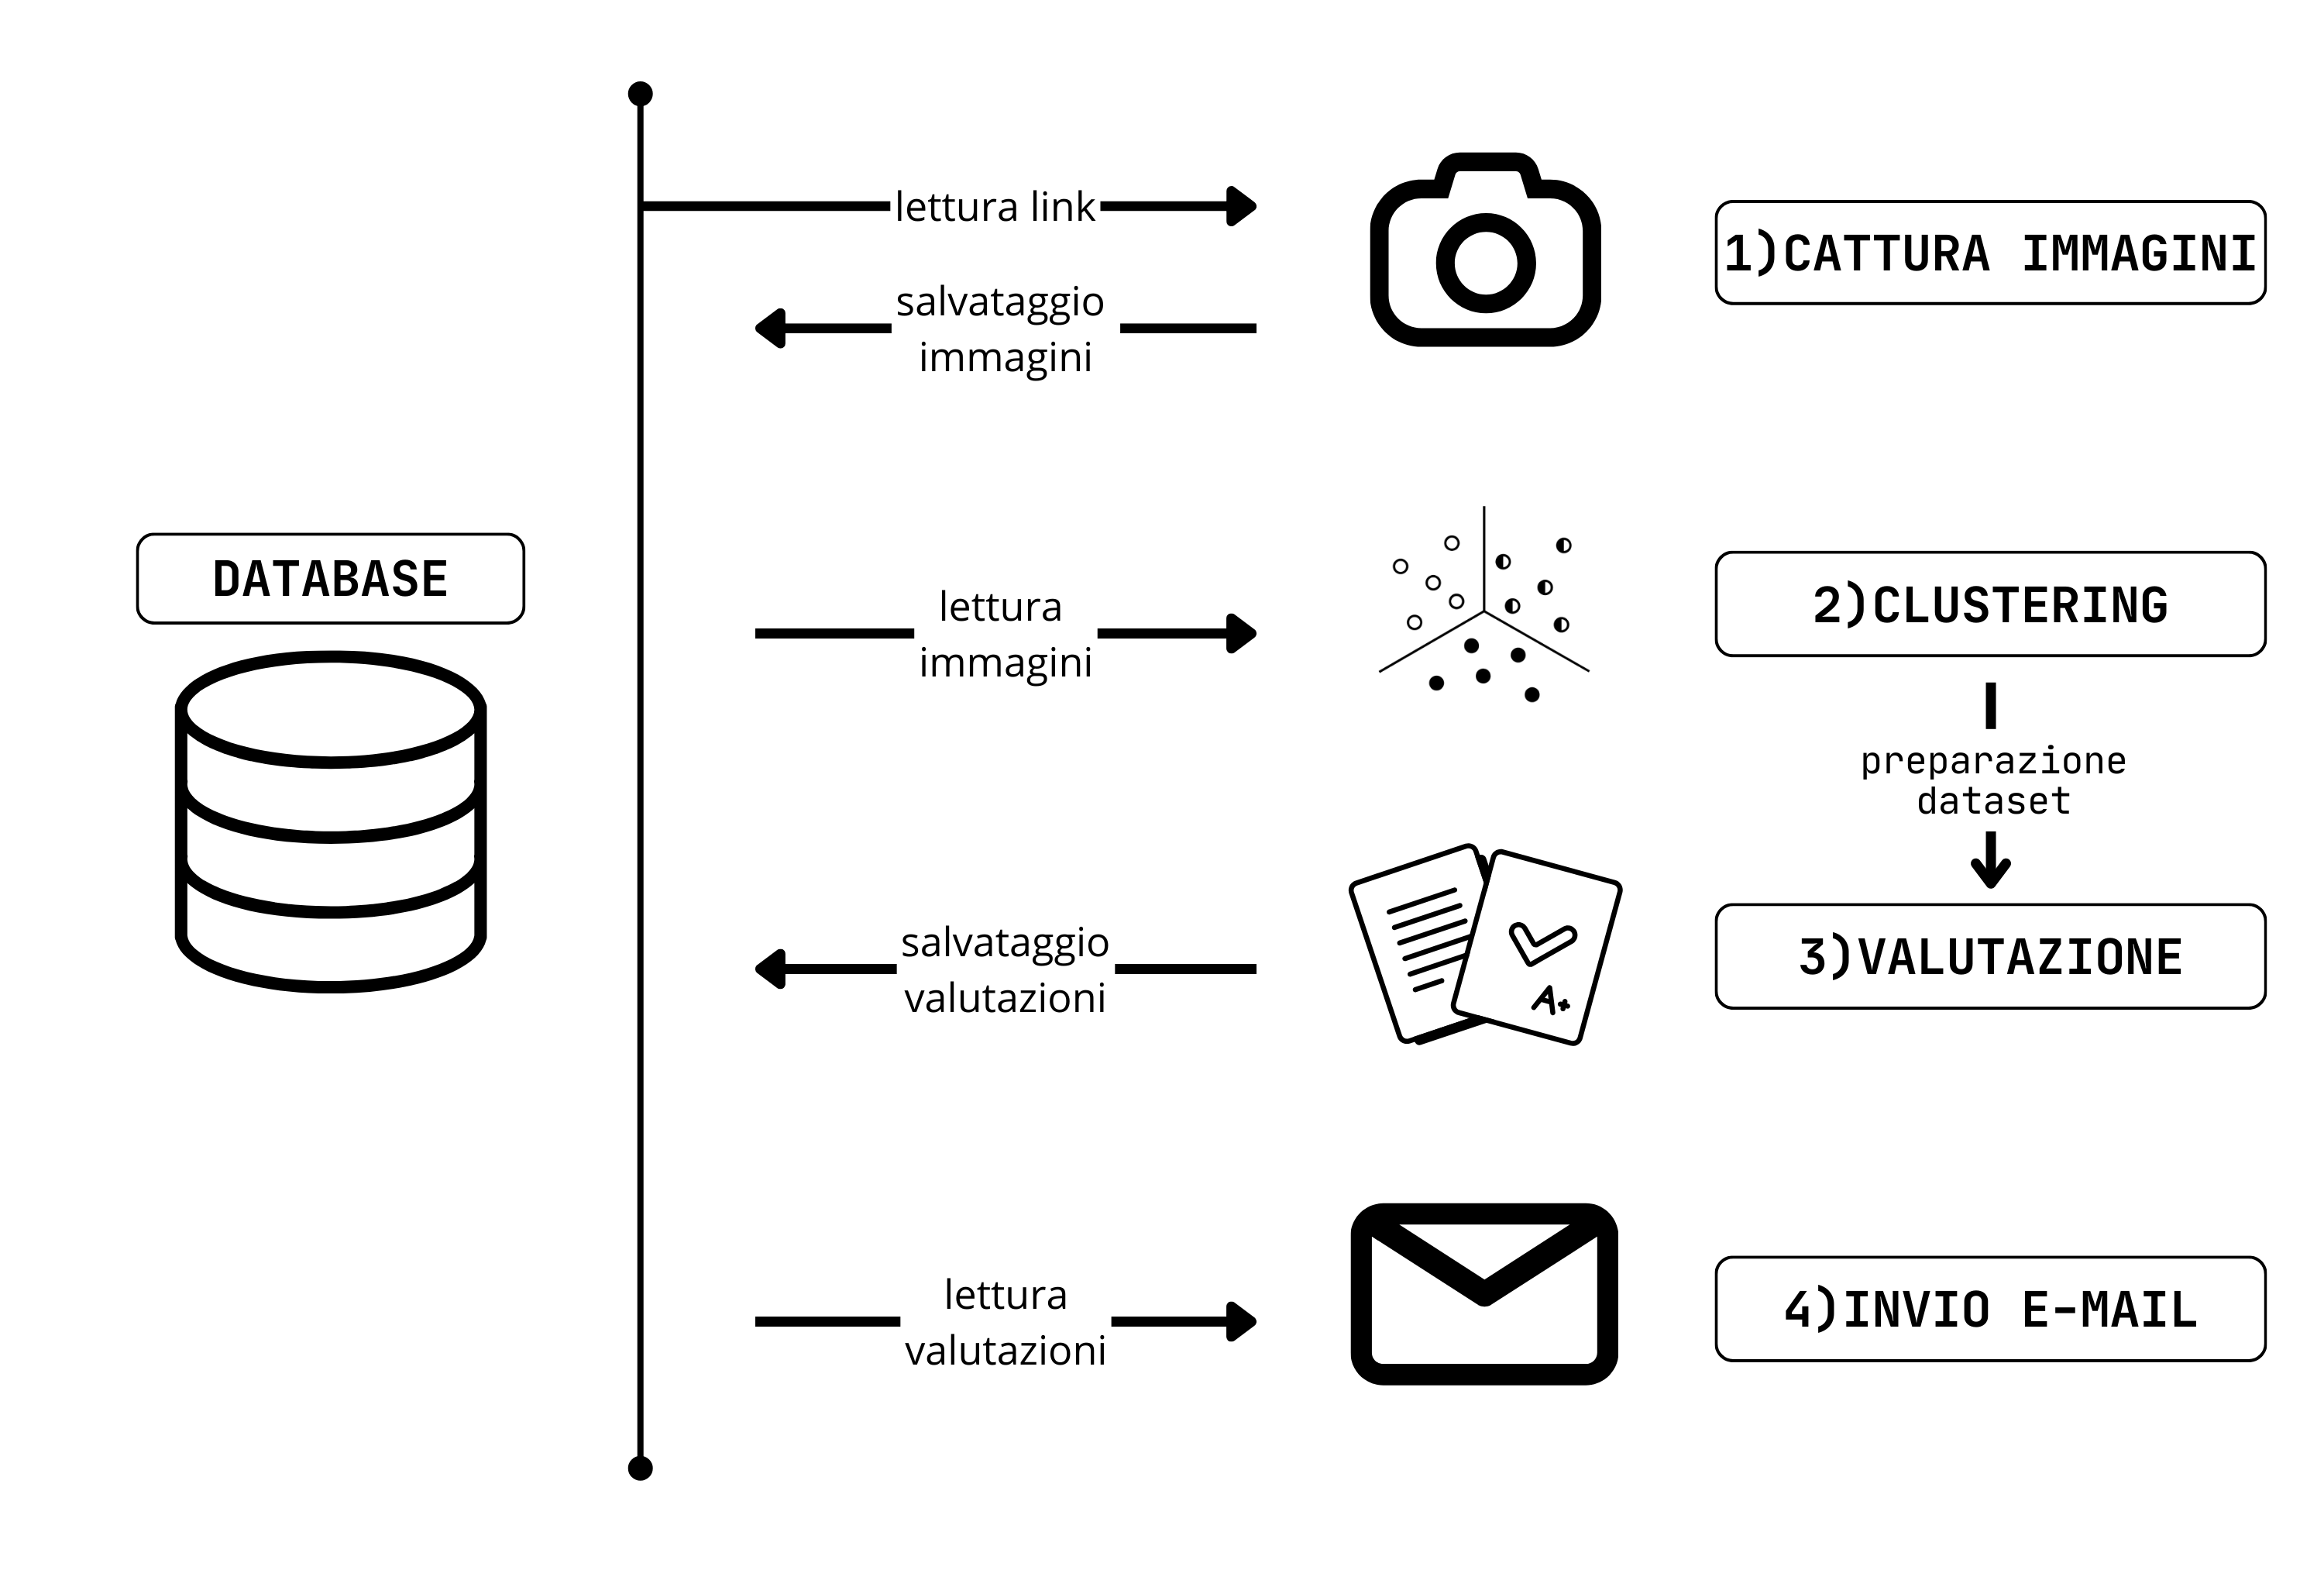
\includegraphics[width=0.9\columnwidth]{progettazione/schema-architettura.png} 
    \caption{Schema architetturale del progetto}
    \label{fig:schema-architettura}
  \end{figure}


\newpage

\section{Cattura immagini}
La prima fase del workflow (Fig.~\ref{fig:schema-cattura}) è composta da uno script Python che usufruisce della libreria Pyppeteer per acquisire gli screenshot dei siti contenuti nel database.
Più precisamente un web-scraper già implementato raccoglie i link delle pagine web dei clienti potenziali, successivamente li carica nel database di SalesCRM, dove verranno infine letti dallo script.
Per funzionare Pyppeteer necessita di chromium, dopo aver effettuato il controllo per verificare se esso sia presente o meno procede con la lettura dei link. 
L'automazione apre ogni indirizzo, aspetta qualche secondo e scatta uno screenshot. 
Tutte le immagini vengono poi convertite in formato Base64 e salvate nel database.

\begin{figure}[!h] 
  \centering 
  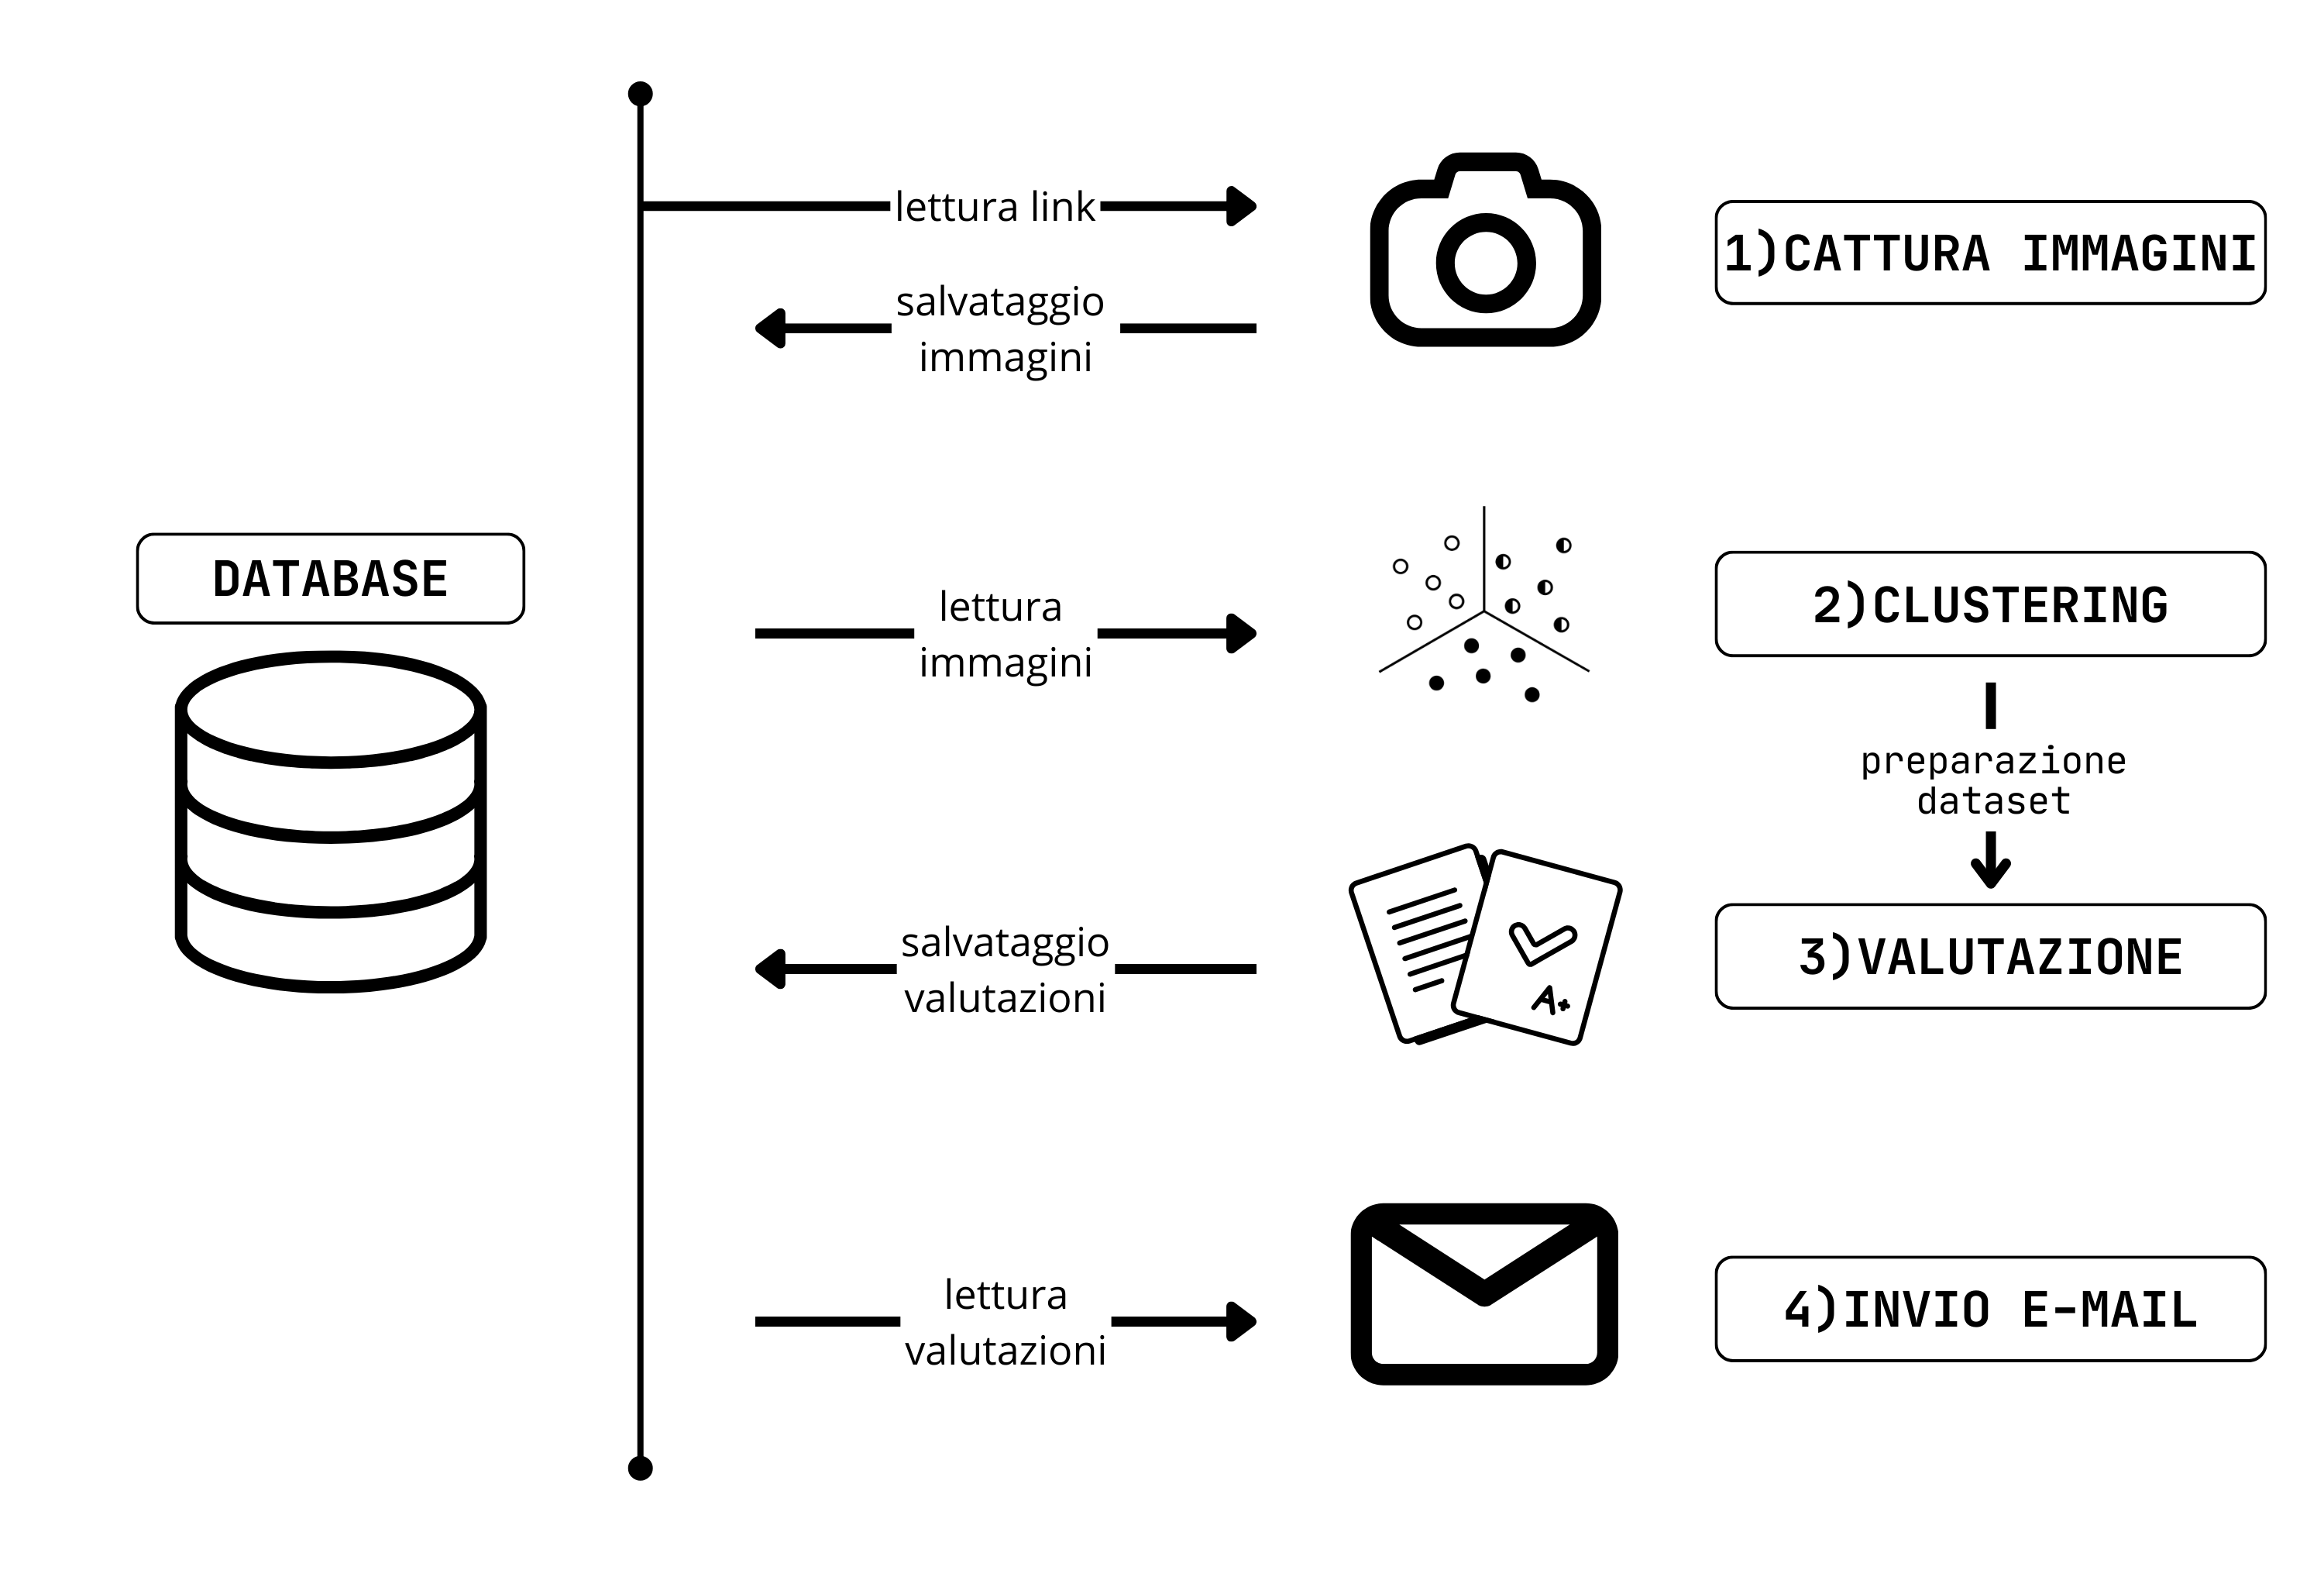
\includegraphics[width=0.9\columnwidth]{progettazione/schema-architettura.png} 
  \caption{Schema della fase di cattura}
  \label{fig:schema-cattura}
\end{figure}

\section{Clustering}

\section{Valutazione}

\section{Invio e-mail}

\section{Database}